\chapter{Θεωρητικό Υπόβαθρο}
\label{ch:theoretical_background}

\section{Πλέγματα}
\begin{wrapfigure}{r}{0.25\textwidth}
    \centering
    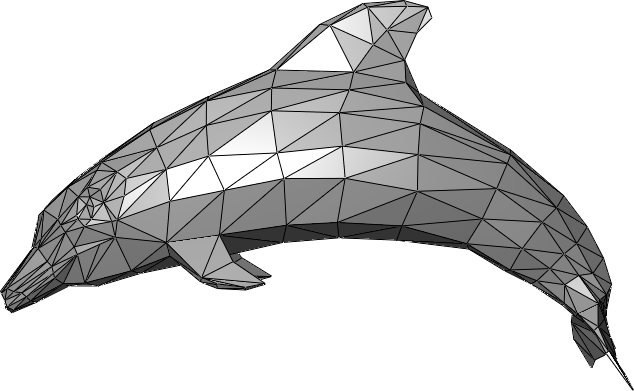
\includegraphics[width=0.25\textwidth]{Dolphin_triangle_mesh.png}
    \caption[Παράδειγμα Τριγωνικού Πλέγματος]{
        Παράδειγμα τριγωνικού πλέγματος που αναπαριστά ένα δελφίνι.
    }
    \label{fig:example_mesh}
\end{wrapfigure}
\label{sec:triangle_meshes}
Στην Υπολογιστική Γεωμετρία τα πλέγματα αποτελούν την αναπαράσταση
μιας μεγαλύτερης γεωμετρικής περιοχής από μικρότερα διακριτά στοιχεία.
Τα πλέγματα χρησιμοποιούνται συνήθως για τον υπολογισμό λύσεων μερικών 
διαφορικών εξισώσεων, για την απόδοση γραφικών υπολογιστών, και για
ανάλυση γεωγραφικών και χαρτογραφικών δεδομένων.
Ένα πλέγμα χωρίζει τον χώρο σε μικρότερα στοιχεία (πολύγωνα ή πολύεδρα) όπου
μπορούν να λυθούν οι εξισώσεις, το οποίο στη συνέχεια προσεγγίζει τη λύση 
στο ευρύτερο πεδίο. 
Τα πλέγματα που αποτελούνται από πολύεδρα αντιπροσωπεύουν ρητά τόσο την 
επιφάνεια όσο και τον όγκο ενός αντικειμένου, ενώ τα πολυγωνικά 
πλέγματα αντιπροσωπεύουν μόνο την επιφάνεια (ο όγκος υπονοείται).
Για το πρόβλημα υπολογισμού της Ευκλείδειας απόστασης, ενδιαφερόμαστε 
μόνο για την εξωτερική επιφάνεια των αντικειμένων του τρισδιάστατου χώρου. 

Ένας τύπος πολυγωνικών πλεγμάτων είναι τα τριγωνικά πλέγματα 
(σχήμα \ref{fig:example_mesh}).
Αποτελούνται από ένα σύνολο τριγώνων στις τρεις διαστάσεις, 
τα οποία συνδέονται με τις κοινές τους ακμές ή κορυφές. 
Γεωμετρικά, ένα πλέγμα είναι μια τμηματικά επίπεδη επιφάνεια.
Η τελευταία ιδιότητα ισχύει πάντοτε για τα τριγωνικά πλέγματα.

Υπάρχουν διάφοροι τρόποι για την αποθήκευση ενός τριγωνικού πλέγματος 
στη μνήμη του υπολογιστή. 
Υπάρχουν επίσης μέθοδοι μετατροπής του ενός 
τρόπου αποθήκευσης σε έναν άλλο.
Ενδεικτικά αναφέρουμε την αποθήκευση με:
\begin{itemize}
    \item \textbf{Σετ τριγώνων}: 
    Το πλέγμα αναπαρίσταται απλά από τα τρίγωνα 
    του. 
    Δηλαδή αποθηκεύονται οι συντεταγμένες των κορυφών κάθε τριγώνου.
    \item \textbf{Σετ Τριγώνων με δείκτες}: 
    Το πλέγμα αναπαρίσταται από ένα σετ
    κόμβων και ένα σετ από τριπλέτες με δείκτες στους κόμβους.
    Η κάθε τριπλέτα αναπαριστά ένα τρίγωνο.
    \item \textbf{Λωρίδες Τριγώνων}: 
    Η αποθήκευση αυτή βασίζεται στο γεγονός ότι 
    δύο γειτονικά τρίγωνα μοιράζονται τη μία τους πλευρά. Αυτός 
    ο τρόπος χρησιμοποιείται για συμπίεση των πλεγμάτων.
    \item \textbf{Δομή Τρίγωνου-Γείτονα}: 
    Υποστηρίζει ερωτήματα γειτνίασης τριγώνων.
    \item \textbf{Δομή \tl{Winged-Edge}}: 
    Αποθηκεύει δεδομένα κόμβων, ακμών και όψεων.
    Επιτρέπει εύκολη διάβαση στο πλέγμα μεταξύ όψεων, ακμών και κορυφών.
\end{itemize} 
Για τους αλγορίθμους που περιγράφουμε παρακάτω αρκεί ο πρώτος τρόπος 
αναπαράστασης. 

Τέλος, για τις διάφορες εφαρμογές που χρησιμοποιούνται, τα πλέγματα 
χαρακτηρίζονται και από την ποιότητα τους. Οι πιο συνηθισμένες μετρικές 
ποιότητας είναι:
\begin{itemize}
    \item \textbf{Λοξότητα (\tl{Skewness})}: \\
    Η λοξότητα είναι ο λόγος της απόκλισης μεταξύ του βέλτιστου μεγέθους
    στοιχείου προς στο υπάρχον μέγεθος στοιχείου. 
    Το εύρος της λοξότητας είναι μεταξύ 0 (ιδανικό) έως 1 (χειρότερο).
    Τα πολύ λοξά στοιχεία δεν προτιμώνται λόγω της κακής ακρίβειας 
    που προκαλούν στις παρεμβαλλόμενες περιοχές.
    Ανάλογα με το στοιχείο (τρίγωνο, τετράπλευρο, τετράεδρο, 
    εξάεδρο κλπ) διαφοροποιείται μαθηματικός τύπος 
    για τον υπολογισμό της λοξότητας.

    \item \textbf{Ομαλότητα (\tl{Smoothness})}: \\
    Η αλλαγή στο μέγεθος των στοιχείων πρέπει να είναι ομαλή. 
    Συνήθως αποφεύγονται ξαφνικά άλματα στο μέγεθος των στοιχείων γιατί αυτό 
    μπορεί να προκαλέσει λανθασμένα αποτελέσματα σε κοντινούς κόμβους.
    
    \item \textbf{Αναλογία Διαστάσεων (\tl{Aspect Ratio})}: \\
    Εν συντομία, ο λόγος διαστάσεων είναι ο λόγος του μεγαλύτερου μήκους 
    ενός στοιχείου προς το μικρότερο μήκος. 
    Ο ιδανικός λόγος διαστάσεων είναι 1. 
    Όσο μικρότερος είναι, τόσο υψηλότερη είναι η ποιότητα ενός στοιχείου. 
    Η μέθοδος υπολογισμού ποικίλλει ανάλογα με τον τύπο κελιού.
\end{itemize}

Σε πραγματικές εφαρμογές, τα πλέγματα συνήθως σχεδιάζονται έτσι ώστε 
να μην παραβιάζουν σε μεγάλο βαθμό τις παραπάνω μετρικές ποιότητας.
Αυτή η παρατήρηση είναι χρήσιμη για τον σχεδιασμό της δομής δεδομένων 
που προτείνουμε.

\begin{figure}[h]
    \centering
    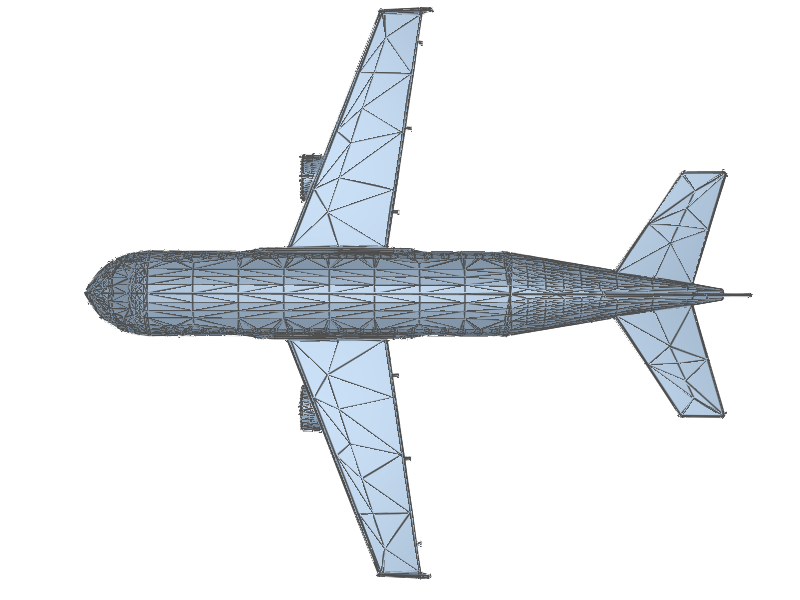
\includegraphics[width=0.45\textwidth]{airplane_bad_mesh.png}
    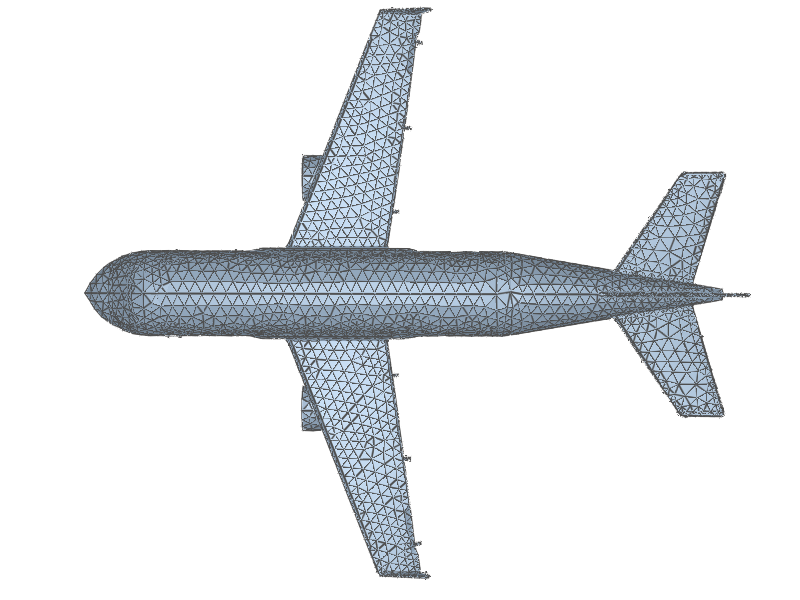
\includegraphics[width=0.45\textwidth]{airplane_good_mesh.png}
    \caption[Παράδειγμα Ποιότητας Πλεγμάτων]{
        Παράδειγμα Ποιότητας Πλεγμάτων - Και τα δύο πλέγματα 
        αναπαριστούν το ίδιο αεροπλάνο. Το δεξί πλέγμα είναι 
        καλύτερης ποιότητας από το αριστερό που φαίνεται να 
        παραβιάζει όλα τα κριτήρια ποιότητας που αναφέρθηκαν
        (\tl{skweness, smoothness, aspect ratio}).
    }
\end{figure}




\section{Ευρετήρια για Χωρικά Δεδομένα}

\section{Οριοθετικοί Όγκοι}
\subsection{Οριοθετικά Πλαίσια Ευθυγραμμισμένα με τους Άξονες}

\section{Ιεραρχίες Οριοθετικών Όγκων}
